\documentclass[12pt, a4paper]{article}
\usepackage[utf8]{inputenc}
\usepackage[T1]{fontenc}
\usepackage[slovene]{babel}
\usepackage{lmodern}
\usepackage{amsmath}
\usepackage{units}
\usepackage{eurosym}
\usepackage{amsfonts}
\usepackage{fancyhdr,amssymb,amsmath,amsthm,bbm,enumerate,mdwlist,url,multirow,hyperref,graphicx}
\usepackage{pdfpages}
\usepackage{comment}
\usepackage{breqn}
\usepackage{caption}
\usepackage{subcaption}
\usepackage{float}
\usepackage{graphicx}


\usepackage{enumerate}
\setlength{\parindent}{0mm}

\DeclareUnicodeCharacter{2212}{-}

\begin{document}
\begin{titlepage}
\begin{center}

\large
Univerza v Ljubljani\\
\normalsize
Fakulteta za matematiko in fiziko\\

\vspace{5 cm} 

\large
Finančni praktikum \\


\vspace{0.5cm}
\LARGE
\textbf{Stable roommate problem}

\vspace{0.5 cm}

\large
Timotej Giacomelli in Nejc Duščak\\


\vspace{1.5cm}
\normalsize
Mentorja: prof. dr. Sergio Cabello, asist. dr. Janoš Vidali
\vspace{3cm}


\vfill

\large Ljubljana, 2020

\end{center}
\end{titlepage}


\newpage

\tableofcontents
\vspace{22mm}

\newpage

\section{Opis problema}
\textit{Stable roommate problem}, znan tudi kot kratica \textbf{SR}, je eden izmed \textit{stable matching} problemov. Problem je dobil ime zaradi svoje praktične uporabe - kako razporediti ljudi v dvoposteljne sobe, glede na njihove preference.\\

Problem je sestavljen iz $2n$ "udeležencev", kjer ima vsak udeleženec seznam preferenc s $2n - 1$ elementi, torej po eno vrednost za vsakega soudeleženca. Vsak udeleženec predstavljen točko v metričnem prostoru, njegov seznam pa so urejene dolžine do ostalih soudeležencev.\\

Ujemanje je množica $n$ disjunktnih parov udeležencev.
Za ujemanje $M$ je par $\{m_{1}, m_{1}' \} \notin M$ \textit{blocking pair}, če zadošča naslednjim pogojem:
\begin{itemize}
	\item  $\{m_{1}, m_{1}' \}, \{m_{2}, m_{2}' \} \in M$,
	\item $m_1$ preferira $m_2$ bolj kot $m_1'$,
	\item $m_2$ preferira $m_1$ bolj kot $m_2'$.
\end{itemize}
Oziroma če povemo z besedami, \textit{blockin pair} nastane, če se imata vsaj dva udeleženca, ki nista v paru, pri ujemanju raje, kot s svojim partnerjem.
Ujemanje $M$ je nestabilno, če zanj obstaja \textit{blocking pair}. Drugače je ujemanje $M$ stabilno.\\

V projektu  sva obravnavala enostavnejšo verzijo osnovnega problema, in sicer \textit{Geometric stable roomate problem}. V tem problemu so udeleženci predstavljeni kot točke v ravnini, kjer lahko te točke izberemo iz poljubno omejenega območja ali pa jih izbiramo kar iz celotne ravnine. V najinem projektu sva na začetku točke izbirala iz kvadrata velikosti 1x1. Preference so tukaj zelo preproste, saj so podane le kot razdalja do točk, kjer manjša razadlja do točke pomeni večjo preferenco. V tem problemu želiva poiskati stabilne pare, ki ustrezajo seznamu preferenc. \\

\begin{center}
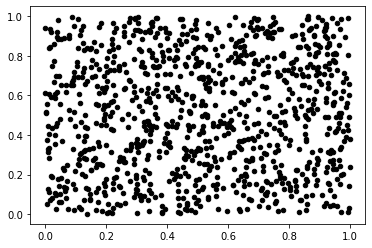
\includegraphics{rdece_tocke.png}
\end{center}


\section{Glavne ideje problema in psevdokoda}
Točke v kvadratu sva določila tako, da sva generirala x in y koordinato posamezne točke in jih shranila v \textit{slovar točk}, kjer ključ slovarja predstavljajo ime točke (npr. \textit{tocka_0}), vrednost pa koordinate točke. Vrednosti slovarja so oblike (\textit{x,y}). V nadaljevanju projekta bova poskusila točke izbirati tudi iz območij drugačne oblike, če bo le možno tudi točke iz neomejenega območja.\\

Razdalje med točkami sva izračunala s pomočjo Pitagorovega izreka. S funkcijo \textit{for} sva se sprehodila čez vse ključe v \textit{slovarju točk} in oblikovala novi slovar imenovan \textit{slovar razdalj}, v katerem je ključ slovarja ponovno ime točke, vrednosti pa vsebujejo seznam razdalj do posameznih točk. Prvotno sva računanje Pitagorovega izreka  razdelila na 3 podprimere. Kasneje sva našla hitrejši način, ki za izračun razdalje porabi manj časa.\\
V nadaljevanju sva s pomočjo funkcije \textit{preference} uredila \textit{slovar razdalj} glede na razdaljo. Tako sva dobila seznam tuplov, urejen po velikosti od najkrajše do najdaljše razdalje.  \\

Do sedaj sva zgenerirala slovar v katerem imava vse točke in urejen seznam preferenc.  V tem delu projekta pa nastopi reševanje problema. Ideja reševanja problema je bila, da bi se sprehodila čez vse točke v slovarju in pri vsaki točki preverila njene preference. Ko bi našla najkrajšo razdaljo med dvema točkama, bi ti dve točki povezala v par in posledično na koncu pridobila ujemajoče pare. Algoritem za reševanje te ideje pa sva sestavila iz dveh funkcij:
\begin{itemize}
	\item najprej sva sestavila funkcijo \textit{Najkrajsa}, ki poišče najkrajšo razdaljo med vsemi točkami. Sprehodimo se po vseh točkah in preverimo njihove prve preference. Ko najdemo najmanjšo oziroma najkrajšo razdaljo, funkcija izbere tisti dve točki, med katerima ta razdalja nastopi in ju poveže v par. Na koncu nam vrne par točk, s pripadajočo najmnajšo razdaljo,
	\item druga funkcija \textit{Vsi_pari}, pa nam omogoča, da kličemo funkcijo \textit{Najkrajsa} dokler ne povežemo vse točke v paru. Pomembno je tudi omeniti, da ko najdemo povezavo med dvema točkamo, potem ti dve točki zbrišemo tako iz slovarja, kot tudi iz seznama preferenc drugih točk, saj tako dosežemo, da se funkcija hitreje konča.
\end{itemize}


\section{Robni pogoji}
V procesu preverjanja pravilnosti algoritma, sva definirala tri "robne primere", v katerih bi lahko prišlo do težav z algoritmom. Pomembno je omeniti, da so vsi primeri narejeni le za točke, ki so generirane v kvadratu. Ti primeri so:
\begin{itemize}
\item Točke so razporejene v kvadrat:\\
	primer_1 = \{'tocka_0': (0.1, 0.1), 'tocka_1': (0.2, 0.1),  'tocka_2': (0.1,
	0.2),  'tocka_3': (0.2, 0.2)\}


\item Vse točke ležijo na vodoravni premici, kjer je razdalja od levega najbližjega soseda (če obstaja) enaka razdalji do desnega soseda (če obstaja):\\
	    primer_2 = \{'tocka_0': (0.1, 0.1), 'tocka_1': (0.2, 0.1), 'tocka_2': (0.3, 0.1),  'tocka_3': (0.4, 0.1),
           'tocka_4': (0.5, 0.1), 'tocka_5': (0.6, 0.1), 'tocka_6': (0.7, 0.1),  'tocka_7': (0.8, 0.1),
           'tocka_8': (0.9, 0.1), 'tocka_9': (1, 0.1)\}

\item Razširjen primer_1 na 12 točk.\\


\end{itemize} 

\pagebreak
\section{Eksperimentiranje z algoritmom}
Za eksperimentiranje z najinim algoritmom sva si izbrala računanje vsote razdalj med točkami v izbranem območju in preverila kako se vsota obnaša glede na število izbranih točk in glede na izbrano območje. Za ta namen sva sestavila funkciji \textit{vsota_razdalj} in \textit{razlicne_vsote}. Funkcija  \textit{vsota_razdalj} sešteje razdalje med točkami, ki so povezane v par. Funkcijo \textit{razlicne_vsote} pa sva sestavila z namenom, da opazujeva kako se obnašajo vsote, ko povečujemo število točk. \\

\subsection{Eksperimentiranje v kvadratu velikosti 1x1}
Pri opazovanju gibanja števila vsote sva dobila spodnjo funkcijo.\\
\begin{center}
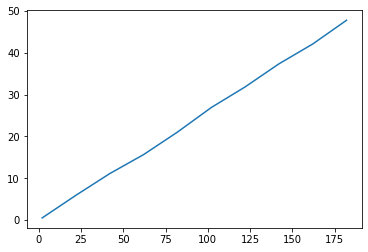
\includegraphics{kvadrat_1x1.png}
\end{center}
Opazimo lahko, da vsote naraščajo skupaj s številom točk. Seveda v nekaterih primerih prihaja do manjših odstopanj, vendar je opazno, da vsote rastejo.

\newpage

\subsection{Eksperimentiranje v krogu s polmerom $r$}
V drugem primeru sva definirala točke znotraj kroga s polmerom $r$, kjer sva polmer $r$ izbrala na začetku. Tu lahko eksperimentiramo na več različnih načinov.
Na primer povečujemo število izbranih točk pri dani izbiri $r = 1$.
\begin{center}
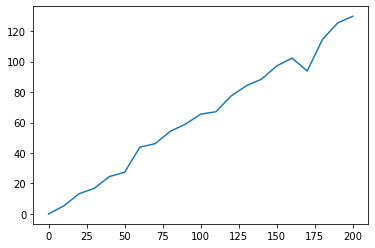
\includegraphics{krog_s_danim_polmerom.png}
\end{center}
Opazimo, da tudi v tem primeru vsote rastejo enakomerno z višanjem števila izbranih točk.
	
\newpage

\subsection{Eksperimentiranje s kvadratom in krogom}
V tem razdelku sva opazovala, kako različni območji (v najinem primeru kvadrat in krog), ki ima enako ploščino, vplivata na vsoto razdalj vseh točk v paru. Za ta primer sva si izbrala kvadrat velikosti $1$x$1$, na drugi strani pa sva izbrala krog s polmerom $ r=\dfrac{1}{\sqrt{\pi}}$. Tako sva dobila območji, ki imata enako ploščino.\\

Na sliki so z rdečo barvo označene vsote točk, ki ležijo v kvadratu, z modro pa točke, ki ležijo v krogu.\\
\begin{center}
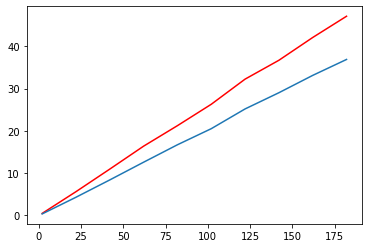
\includegraphics{primerjava_krog_kvadrat.png}
\end{center}
Opazimo lahko, da so vsote večje v kvadratih kot v krogih.\\


\subsection{Eksperimentiranje s kocko in sfero}
Za konec pa sva pogledala še območja oblike treh dimentzij (3D). Najprej sva se lotila  kocke z robom dolžine 1. Videla sva, da se tudi v tem primeru vsote povečujejo skupaj z večanjem števila točk.\\
Enako sva ponovila na sferi z enakim volumnom kot pri kocki. Gibanje vsot za oba primera je prikazano na spodnji sliki, kjer rdeča črta označuje vsote razdalj v kocki, modra pa vsote v sferi.
\begin{center}
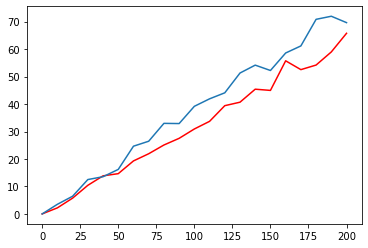
\includegraphics{primerjava_kocka_sfera.png}
\end{center}
Vidimo, da so tudi v treh dimenzijah vsote razdalj, med točkami v paru, v kocki večje od vsot razdalj v sferi.


\end{document}


